\documentclass[a4paper,	11pt]{article}

% add latex preamble
% para la bibliografía se requiere biber y configurar texstudio

% Latex packages
\usepackage[utf8]{inputenc}
\usepackage[T1]{fontenc} % para copiar acentos en español del pdf y permite acentos en las notas
\usepackage[spanish]{babel}
\usepackage[per-mode = symbol]{siunitx} % para manejar las unidades
\usepackage{multimedia} % to add videos with \movie command
\usepackage{multirow}
\usepackage{graphicx}
\usepackage{xcolor}
\usepackage{amsmath} % bmatrix
\usepackage[makeroom]{cancel} % \cancel to cancel terms in math equations
\renewcommand{\CancelColor}{\color{red}} % set red color for \cancel command
\usepackage[caption=false]{subfig} % caption = false elimina la palabra "Figura" del caption
\usepackage{import} % para el comando import (se usa para pdf_tex)
\captionsetup[subfigure]{labelformat=empty} % remover el indice del caption de la subfigura
\usepackage{booktabs} % \toprule \midrule \bottomrule
\usepackage[backend=biber]{biblatex} % set biber to format references. Must configure Biber in Texstudio
\usepackage{csquotes} % to remove warning triggered by biblatex and babel
\usepackage{algorithm} % to put captions to the algorithmics environmets
\usepackage{algpseudocode} % to write algorithm
\usepackage{tikz} % to use tikz
\usepackage[export]{adjustbox} %valign in subfloat
\usepackage{colortbl} % to paint cells in a table
\usepackage{todonotes} % add latex todo notes

% Color commands for annotations
\newcommand\TODO[1]{\textbf{\textcolor{red}{#1}}} %  TODO notes

% Graphic paths
\graphicspath{{./images/}}

% listings configuration for C code
\usepackage{listings} % code
\definecolor{commentgreen}{RGB}{2,112,10}
\definecolor{eminence}{RGB}{108,48,130}
\definecolor{weborange}{RGB}{255,165,0}
\definecolor{frenchplum}{RGB}{129,20,83}

\lstset{ % spanish characters for listings package
	inputencoding=latin1,
    columns=fullflexible,
	breaklines=true,
	tabsize=2,
	showstringspaces=false,
	basicstyle=\ttfamily,
	backgroundcolor=\color{lightgray}, % Choose background color
	literate={á}{{\'a}}1
	{ã}{{\~a}}1
	{é}{{\'e}}1
	{ó}{{\'o}}1
	{í}{{\'i}}1
	{ñ}{{\~n}}1
	{¡}{{!`}}1
	{¿}{{?`}}1
	{ú}{{\'u}}1
	{Í}{{\'I}}1
	{Ó}{{\'O}}1
    {-}{-}1
}

\lstdefinestyle{cpp}{ % spanish characters for listings package
    language=C++,
   	commentstyle=\color{commentgreen},
    keywordstyle=\color{eminence},
    stringstyle=\color{red},
    emph={int,char,double,float,unsigned,void,bool},
    emphstyle={\color{blue}}
}

\lstdefinestyle{bash}{ % spanish characters for listings package
	language=Bash
}

\lstdefinestyle{xml}{
	language=XML,
	morekeywords={encoding,xs:schema,xs:element,xs:complexType,xs:sequence,xs:attribute}
}

\lstdefinestyle{cmake}{
	language=make, % there is no cmake support in listings
}

\lstdefinestyle{python}{
    language=python,
}


%%%%% PARA QUE EN LAS TABLAS SE PUEDA PONER UN SALTO DE LINEA DENTRO DE UNA CELDA
\newcommand{\specialcell}[2][c]{%
    \begin{tiny}
        \begin{tabular}[#1]{@{}c@{}}#2\end{tabular}  
    \end{tiny}
}
%%%%%%%%%%%%%%%%%%%%%%%%%%%%%%%%%%%%%%%%%%%%%%%%%%%%%%%%%%%%%%%%%%%%%%%%

%%%%% PARA QUE LAS TABLAS TENGAN TODAS LAS COLUMNAS CENTRADAS Y DE IGUAL TAMAÑO
\usepackage{tabularx}
\renewcommand{\tabularxcolumn}[1]{>{\centering\arraybackslash}m{#1}}
%%%%%%%%%%%%%%%%%%%%%%%%%%%%%%%%%%%%%%%%%%%%%%%%%%%%%%%%%%%%%%%%%%%%%%%%



% add math preamble
\usepackage{amsmath}
\usepackage{amssymb}
\usepackage{amsopn}
\usepackage{mathtools}
\usepackage{nicematrix} % Add colors to matrix


% set matrix maximum length
\setcounter{MaxMatrixCols}{20}

% math
\renewcommand{\vec}[1]{\boldsymbol{\mathbf{#1}}}
\newcommand{\norm}[1]{\lVert#1\rVert}

% Declare arg max and arg min functionss
\DeclareMathOperator*{\argmax}{arg\,max}
\DeclareMathOperator*{\argmin}{arg\,min}

% Declare atan2 
\DeclareMathOperator{\atantwo}{atan2}

% Homogeneous decoration function
\newcommand{\homo}[1]{\dot{#1}}


% Declare projection as math function
\DeclareMathOperator{\proj}{proj}
\newcommand{\fromCoord}[2]{{#1}_\mathrm{#2}}
\newcommand{\toCoord}[2]{\prescript{\mathrm{#2}}{}{#1}}
\newcommand{\worldCoordSystem}{\mathrm{W}}
\newcommand{\bodyCoordSystem}{\mathrm{B}}
\newcommand{\cameraCoordSystem}{\mathrm{C}}
\newcommand{\origin}{\vec{o}}
\newcommand{\point}{\vec{p}}
\newcommand{\worldPoint}{\toCoord{\point}{\worldCoordSystem}}
\newcommand{\imagePoint}{\vec{u}}
\newcommand{\cameraPoint}{\toCoord{\point}{\cameraCoordSystem}}
\newcommand{\homoWorldPoint}{\toCoord{\homo{\point}}{\worldCoordSystem}}
\newcommand{\homoImagePoint}{\homo{\imagePoint}}
\newcommand{\homoCameraPoint}{\toCoord{\homo{\point}}{\cameraCoordSystem}}
\newcommand{\measurement}{\vec{z}}
\newcommand{\prediction}{\hat{\vec{z}}}
\newcommand{\seMatrix}{\vec{\xi}}
\newcommand{\transform}[2]{\toCoord{\fromCoord{\seMatrix}{#2}}{#1}}
\newcommand{\pointCoord}[1]{\toCoord{\point}{#1}}
\newcommand{\rotation}{\vec{R}}
\newcommand{\rotationCoord}[2]{\toCoord{\fromCoord{\rotation}{#2}}{#1}}
\newcommand{\translation}{\vec{t}}
\newcommand{\translationCoord}[2]{\toCoord{\fromCoord{\translation}{#2}}{#1}}
\newcommand{\intrinsicMatrix}{\vec{K}}
\newcommand{\principalPoint}{\vec{c}}
\newcommand{\reprojectionError}{u}
\newcommand{\projectionMatrix}{\vec{P}}
\newcommand{\cameraCenter}{\vec{o}}
\newcommand{\worldCameraCenter}{\toCoord{\cameraCenter}{\worldCoordSystem}}
\newcommand{\essentialMatrix}{\vec{E}}
\newcommand{\fundamentalMatrix}{\vec{F}}
\newcommand{\inverse}[1]{{#1}^{-1}}
\newcommand{\epipole}{\vec{e}}

% Localization (State Estimation)
\newcommand{\state}{x}
\newcommand{\observation}{z}
\newcommand{\controlCommand}{u}
\newcommand{\covariance}{\Sigma}
\newcommand{\motionModelNoise}{\epsilon}
\newcommand{\measurementModelNoise}{\delta}
\newcommand{\motionModelFunction}[1]{g\left( #1 \right)}
\newcommand{\observationModelFunction}[1]{h\left( #1 \right)}
\newcommand{\motionParametersCovariance}{R}
\newcommand{\observationModelCovariance}{Q}
\newcommand{\motionModelJacobian}{G}
\newcommand{\observationModelJacobian}{H}
\newcommand{\kalmanGain}{K}
\newcommand{\normalDistribution}[2]{\mathcal{N}\left( {#1}, {#2} \right)}
\newcommand{\motionModelJacobianControl}{V}
\newcommand{\motionModelCovariance}{M}
\newcommand{\stateEvolutionMatrix}{A}

% Mapping slides
\newcommand{\map}{m}
\newcommand{\mapRandomVariable}{m}

% SLAM slides
\newcommand{\informationMatrix}{\vec{\Omega}}
\newcommand{\error}{\vec{e}}
\newcommand{\observationBold}{\vec{z}}
\newcommand{\stateBold}{\vec{x}}
\newcommand{\jacobian}{\vec{J}}
\newcommand{\linearSystemb}{\vec{b}}
\newcommand{\linearSystemH}{\vec{H}}
\newcommand{\covarianceBold}{\vec{\covariance}}


% Motion Planning slides
\newcommand{\workSpace}{\mathcal{W}}
\newcommand{\obstaclesSet}{\mathcal{O}}
\newcommand{\robotInConfiguration}{\mathcal{A}}
\newcommand{\robotConfiguration}{q}
\newcommand{\configurationSpace}{\mathcal{C}}
\newcommand{\freeConfigurationSpace}{\configurationSpace_{free}}
\newcommand{\obstableConfigurationSpace}{\configurationSpace_{obs}}
\newcommand{\goalSet}{\configurationSpace_{goal}}
\newcommand{\startConfiguration}{\robotConfiguration_{I}}
\newcommand{\goalConfiguration}{\robotConfiguration_{G}}
\newcommand{\continuousPath}{\tau}
\newcommand{\motionLaw}{\gamma}
\newcommand{\robotActionSpace}{\mathcal{U}}


% Motion model
\newcommand{\position}{\vec{p}}
\newcommand{\orientation}{\vec{O}}
\newcommand{\orientationQuaternion}{\vec{q}}
\newcommand{\predictedPosition}{\hat{\vec{p}}}
\newcommand{\predictedOrientationQuaternion}{\hat{\vec{q}}}
\newcommand{\linearVelocity}{\vec{v}}
\newcommand{\angularVelocity}{\vec{\omega}}

\DeclareMathOperator{\slerpOp}{slerp}
\newcommand{\slerp}[1]{\slerpOp{\left( #1 \right)}}

% Map structure
\newcommand{\keyframesSet}{K}
\newcommand{\mapPointsSet}{P}
\newcommand{\observedMapPoints}{O}
\newcommand{\covisibilityKeyframes}{CK}
\newcommand{\localMap}{local\_map}

% Bundle Adjutment
\newcommand{\update}{\vec{\delta}}
\newcommand{\incremental}{\hat{\update}}


% Loop Closure names

% scaled operators and letters to fancy view
\newcommand{\sminus}{\scalebox{0.5}[1.0]{$-$}}
\newcommand{\splus}{\scalebox{0.6}[0.6]{$+$}}
\newcommand{\curr}{c}
\newcommand{\sind}[1]{\scalebox{0.6}[0.6]{$#1$}}
\newcommand{\ind}[1]{\scalebox{0.7}[0.7]{$#1$}}

\newcommand{\keyframe}{\vec{K}}
\newcommand{\bowVector}{\vec{v}}
\newcommand{\lcError}{\vec{\Omega}}
\newcommand{\relativeTransformation}{\seMatrix}
\DeclareMathOperator{\interpolate}{interpolate}

\newcommand{\relativeMotion}{\vec{\delta}}
\newcommand{\groundTruth}[1]{{#1}^{*}}

% definición del operador rot()
\DeclareMathOperator{\rotationOp}{rot}
\newcommand{\getRotation}[1]{\rotationOp{\left( #1 \right)}}

\DeclareMathOperator{\translationOp}{trans}
\newcommand{\getTranslation}[1]{\translationOp{\left( #1 \right)}}









% changes margins
\usepackage[a4paper, total={7.5in, 10.6in}]{geometry}


\begin{document}

\title{Gruía de Escritura Científica}
\author{Taihú Pire}




\maketitle

\tableofcontents

Este documento es una guía para hacer propuestas, informes, tesinas, tesis, publicaciones y presentaciones.


\section{Comentarios generales}
%
\begin{itemize}
    \item El documento en \LaTeX~debe compilar sin errores ni warnings.

    \item Ser detallado y claro en el texto, repetir palabras hace que sea fácil de leer.

    \item Redactar de manera formal: no utilizar ``etc'' por ejemplo, en vez utilizar ``entre otros''.

    \item Mantener una terminología. Ejemplo: usar V-SLAM o SLAM visual, no ambas.

    \item Cada capítulo debe tener un texto introductorio que cuente de qué va el capítulo, qué se presenta o describe.
    
    \item Todas las ecuaciones (incluso las que están centradas) deben terminar con punto (.) o con coma (,). En el caso de coma y punto y seguido no debe haber sangría en la oración que sigue a la ecuación.

    \item Usar itálica para texto en inglés.

    \item Para un término en inglés Ej: \emph{keyframe} utilizar itálica únicamente en la primera ocurrencia de la palabra, luego no se usa más itálica para ese término.

    \item Para las unidades o números con unidades utilizar el paquete siunitx de \LaTeX. Ej: \SI{5}{\meter} o \si{\meter} para unidades solas.

    \item Remover citas que no se referencien en el texto, esto hace que el .bib quede más limpio.
\end{itemize}

\section{Estructura General de una Tesina}
Portada\\
Abstract\\
1. Introducción\\
1.1 Motivación\\
1.2 Objetivos\\
1.3 Trabajos publicados durante la tesina (si los hubiere)\\
1.4 Estructura de la tesina\\
2. Trabajo Relacionado\\
3. Conceptos Previos\\
4. Método\\
5. Experimentos $\leftarrow$ \textbf{Este capítulo es el primero que debe escribirse}\\
6. Conclusiones\\
6.1 Trabajo Futuro\\
Apéndices (si los hubiere)\\
Referencias

\subsection{Estructura general de un Abstract}
Cada oración del abstract tiene que decir algo puntual:\\
La 1ra oración puede ser la que pone contexto.\\
La 2da oración habla sobre el problema que se intenta abordar.\\
La 3ra oración describe el método.\\
La 4ta oración de cómo el método es validado.\\
(El abstract de la tesina puede ser un poco más extenso)


\subsection{Comentarios sobre Trabajo Relacionado}
\begin{itemize}
    \item Explicar los trabajos relacionados que se referencian: características principales, ventajas desventajas, etc.
    \item Ver el estado del arte de los papers e inspirarse en ellos. Ver qué trabajos citan y cómo los describen.
\end{itemize}

\subsection{Tratamiento de Figuras}
%
\begin{itemize}
    \item Las figuras deben estar vectorizadas con inkscape\footnote{\url{https://inkscape.org/}} o descargarlas ya vectorizadas (\lstinline{pdf} vectorizado o \lstinline{svg})
    
    \begin{figure}[!htbp]
        \centering
        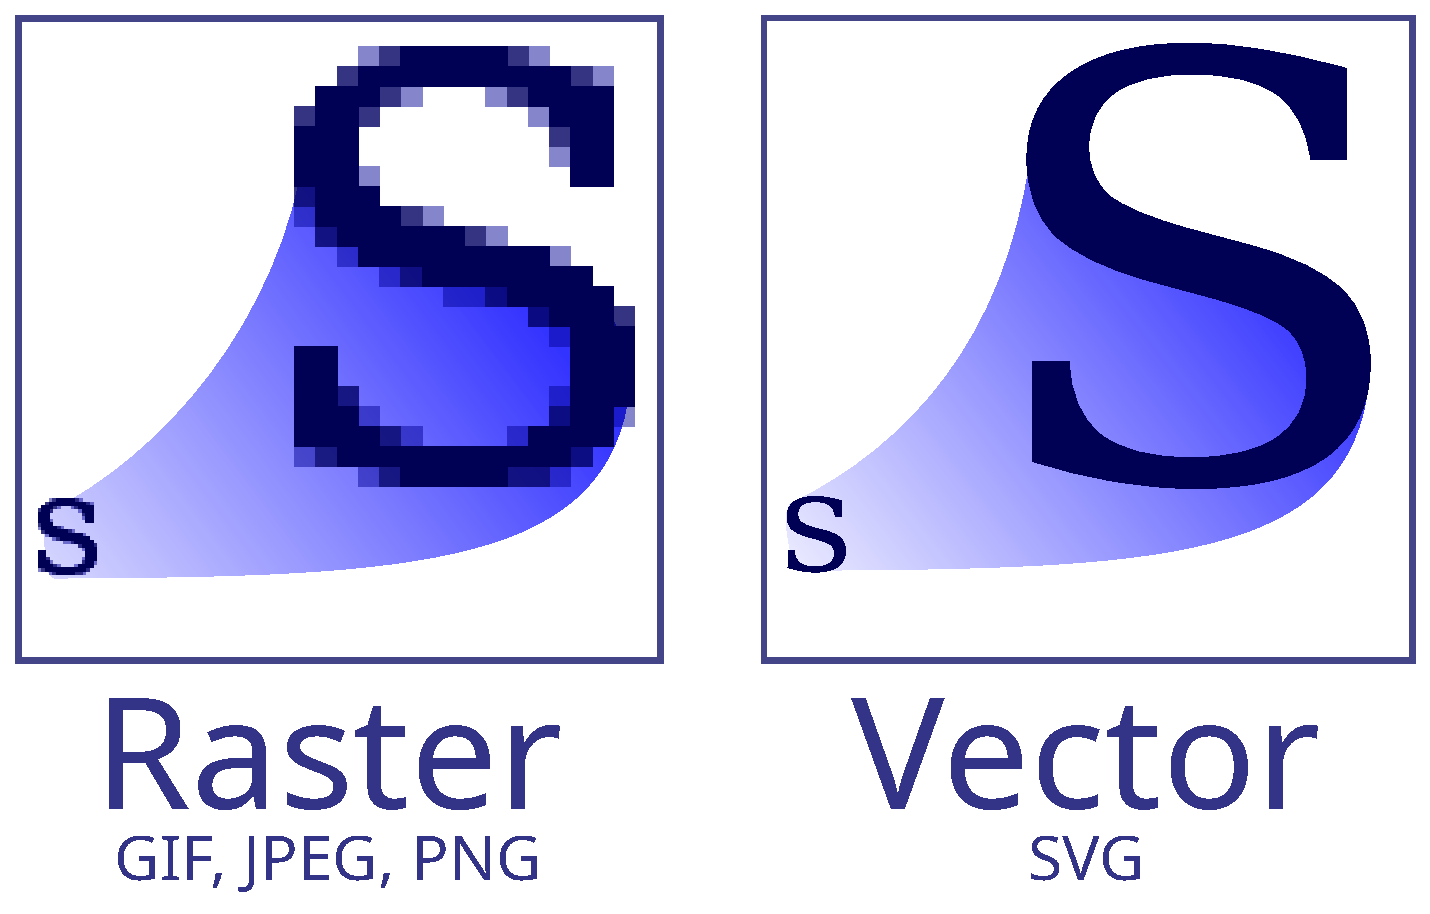
\includegraphics[width=0.5\linewidth]{./images/bitmap_vs_svg.pdf}
        \caption{Diferencias entre imagen raster (jpg, png, tif, entre otros) y vecorizada (pdf vectorizado o svg).}
        \label{fig:bitmap_vs_svg}
    \end{figure}

    \item En inkscape es posible agregar código \LaTeX utilizando plugin \lstinline{textext}\footnote{\url{https://textext.github.io/textext/}}.
    \item En inkscape también se puede poner texto ``normal'' con la tipografía de \LaTeX por defecto que es CMU Serif  (Computer Modern Unicode Serif). Para esto se debe instalar primero el paquete \lstinline{sudo apt-get install fonts-cmu}
    \item En el texto, las figuras siempre se referencian de la misma manera. Ej: La Figura XXX ... Es decir, se las antepone únicamente con la palabra ``Figura''. Observar que la F es mayúscula, y XXX resulta de usar \textbackslash ref\{fig\:nombre\_figura\}.
    \item Todos los captions de las figuras y tablas deben terminar con punto (.)
    \item Cuando una imagen es extraída de un paper sin hacerle modificaciones se debe poner al final del caption la oración: Imagen extraída de [CITA DEL PAPER]. En cambio, si la figura fue modificada o adaptada de [CITA DEL PAPER].
\end{itemize}


\section{Tratamiento de referencias}
Las referencias deben estar formateadas adecuadamente para mantener la formalidad y facilitar su reutilización en otros documentos. Para agregar una cita se debe descargar el bibtex de la página oficial donde esta publicado el trabajo (IEEE, Elsevier, Springer, etc). Agregar el bibtex al \lstinline{.bib}, y luego hacer algunas correcciones:
\begin{itemize}
    \item El keyword único de la referencia debe tener el formato: \lstinline{apellido-primer-autor-año-primera-palabra-del-titulo}. Ej: \lstinline{davison2007monoslam}
    \item Completar el nombre de los autores, casi siempre estan con siglas los nombres, y las letras con acentos no aparecen. Ej: A. Davison -> Andrew Davison o Davison, Andrew
    \item Usar el Keyword definido de la conferencia o revista en el campo ``proceedings'' o ``journal''. Ej: proceedings = ICRA. Acá ICRA es una keyword que es reemplazada por el string ``IEEE Intl. Conf. on Robotics and Automation (ICRA)''
    \item Rodear al título con doble llave para que se mantengan todas las mayúsculas. Ej: title = \{ LALALA \} $\rightarrow$ \{\{ LALALA \}\}
    \item Le agrego un guión extra a las páginas, porque sino no se visualiza bien. Ej: 234-242 $\rightarrow$ 234--242
    \item Siempre debe estar el DOI y/o ISBN de la cita cuando esten disponibles.
\end{itemize}

\section{Herramientas Útiles}

\begin{itemize}
    \item C++/Python
    \item ROS2 (Robotics Operating System): framework de robótica
    \item Gazebo: simulador
    \item Git: versionador
    \item Docker: contenedor
    \item Latex/Lyx: escritura de informes o papers
    \item VScode: IDE de desarrollo
    \item Yed: diagramas \url{https://www.yworks.com/products/yed}
    \item inkscape: gráficos vectorizados + plugin \url{https://textext.github.io/textext/}
    \item pdfpc: visualizador de slides (hechas en latex)
    \item Visualizar Rotaciones \url{https://articulatedrobotics.xyz/tools/rotation-calculator}
    \item Búsqueda y Análisis de papers:
    \begin{itemize}
        \item Búsqueda Avanzada de Google Scholar \url{https://scholar.google.com/}
        \item Mendeley: manejador de papers \url{https://www.mendeley.com/}
        \item \url{https://www.connectedpapers.com/}: grafo para búsqueda del estado del arte
        \item NotebookLM: Ayuda en la comprensión \url{https://notebooklm.google.com/}
    \end{itemize}
\end{itemize}

\end{document}